
\documentclass[11pt]{article}
\usepackage{acl2014}
\usepackage{times}
\usepackage{url}
\usepackage{latexsym}
\usepackage{graphicx}
\usepackage{amsmath}

\DeclareMathOperator*{\argmax}{arg\,max}

%\setlength\titlebox{5cm}

% You can expand the titlebox if you need extra space
% to show all the authors. Please do not make the titlebox
% smaller than 5cm (the original size); we will check this
% in the camera-ready version and ask you to change it back.

\title{Gesture Recognition with Recurrent Neural Networks}

\author{Justin Fu \\
  University of California, Berkeley\\
  {\tt justinfu@berkeley.edu} \\\And
  Siddhartho Bhattacharya \\
  University of California, Berkeley\\
  {\tt siddartho\_b@hotmail.com} \\}

\date{}

\begin{document}
\maketitle 
\begin{abstract}
  Gesture recognition is typically done through images, but it requires
  extensive effort to process image data into a form useful for gesture
  recognition. Our project uses accelerometer data from smartphones,
  so no special hardware is required.
  Recurrent neural networks provide a natural way to model time
  sequences, and the LSTM architecture in particular provides a way
  to model long-range dependencies that are prevalent in
  the gestures we tested. TODO: We imlemented 6 gestures, and achieve an
  accuracy of X percent on the test set we generated.
\end{abstract}

\section{Introduction}

TODO: Intro goes here. Talk about why this problem is
hard/interesting, and possibly some recent work.

Potential applications of this project include making
phones more intuitive to use. For example, imagine 
phones that automatically unlock and lock when you take 
them in and out of your pocket, picking up calls by just
bringing it up to your ear, etc.

\section{Data}

We collected accelerometer data streamed from a smartphone.
Specifically, we only considered values in the X and Y directions
as seen from the perspective of the phone. 

\begin{figure}[ht]
\caption{Directions of each axis on the phone}
  \centering
    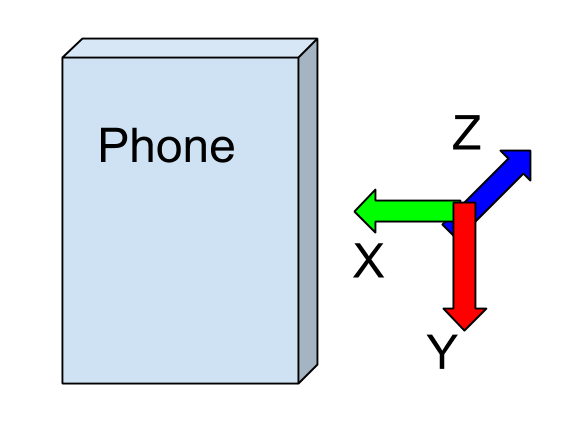
\includegraphics[width=0.5\textwidth]{phone_axis}
\end{figure}

We implemented 6 different gestures representing some letters of
the alphabet (M, Z, O, L, J, and S). Our training set contains
26 instances of each letter and our test set contains 10, for
a total of 216 examples. 

\section{Model}
\label{sect:pdf}

We implemented an LSTM (long short term memory) network based on
the architecture proposed by Graves [1]. Specifically,
our network contains the forget, input, and output gates, but lacks the
peephole connections that connect the internal cell state to these gates
(as done in Vinyals et al. [2]).

\begin{figure}[ht]
\caption{A single LSTM cell. Red arrows are connections forward in time.}
  \centering
    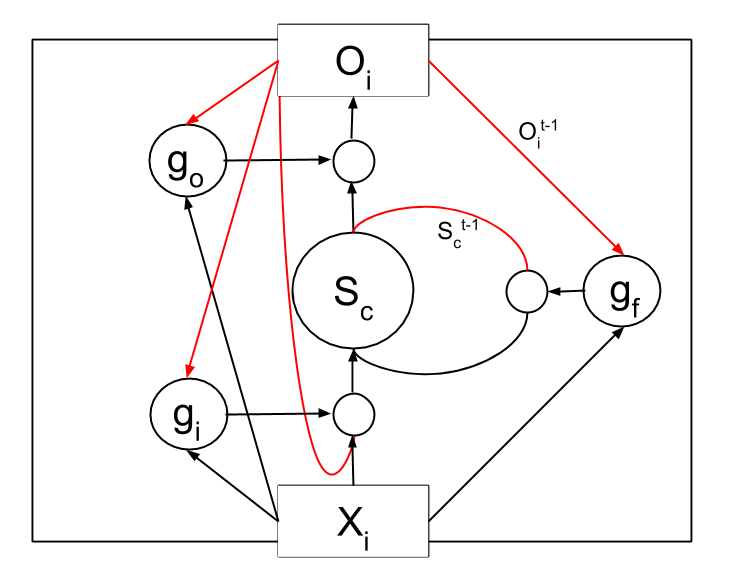
\includegraphics[width=0.5\textwidth]{lstm_cell}
\end{figure}

We then interleave layers of LSTM units with
normal network layers to create a multilayer network.
The output of the final layer is then fed through a softmax function.

\begin{figure}[ht]
\caption{Diagram of one interleaved layer of our network. LSTM 
cells are represented as squares and normal neurons are represented
as circles.}
  \centering
    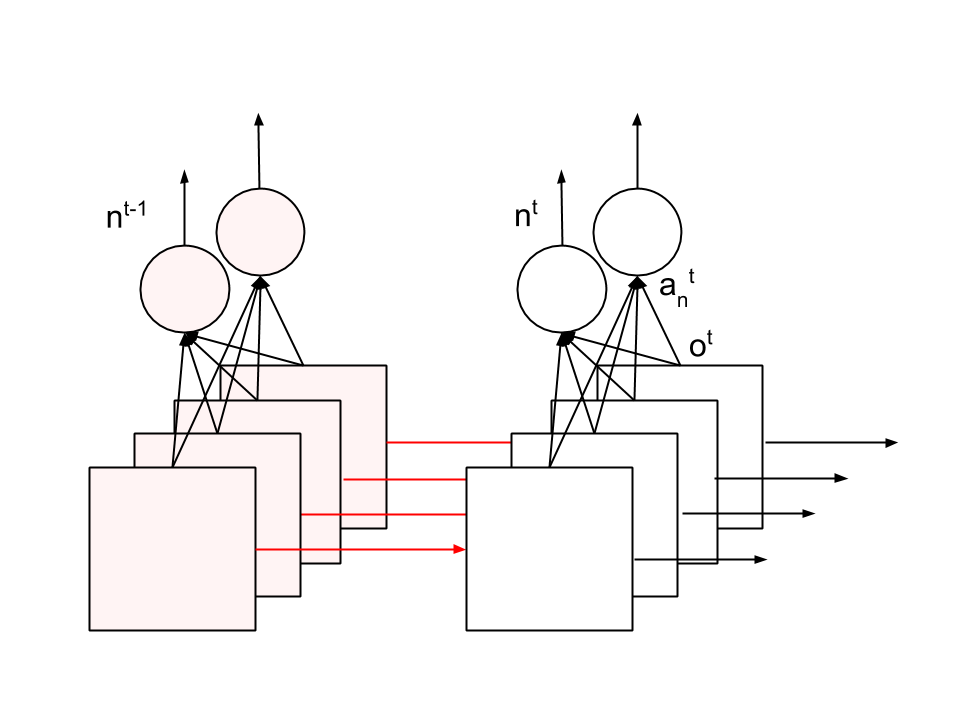
\includegraphics[width=0.5\textwidth]{lstm_network}
\end{figure}

\subsection{Equations}

We used cross-entropy as our objective function. \(O\) is the network
output after the softmax and \(Y\) is the training label. \(n\) sums over each
training example, \(t\) sums over time, and \(i\) sums over the dimensions
of each training example at a given timestep.
Note that \(t\) varies with each training example.

\[  L(Y, O) = \sum_{n}^{N}  \sum_{t}^{len(O^{n})} \sum_{i}^{I} y_{i}^{n,t}*\ln(o_{i}^{n,t}) \]

Most of the equations on the forward and backward passes are the
same as those in Graves [1], but some were missing from his paper
and we dropped the peepholes so we specify all for completeness.

\subsection{Forward Dynamics}
The forward dynamics of the network are specified as follows. Equations
are specified for a whole layer (rather than per unit).
 Bolded values represent vectors. Note that \(*\)
represents a point-wise multiply, and the nonlinearities are applied
element-wise to the input vector.

Gates
\[ \textbf{a}_{i}^{t} = W_{i,x}\textbf{x}^{t} +  W_{i,o}\textbf{o}^{t-1} \] 
\[ \textbf{g}_{i}^{t} = \sigma( \textbf{a}_{i}^{t}) \]
\[ \textbf{a}_{f}^{t} = W_{f,x}\textbf{x}^{t} +  W_{f,o}\textbf{o}^{t-1} \] 
\[ \textbf{g}_{f}^{t} = \sigma( \textbf{a}_{f}^{t}) \]
\[ \textbf{a}_{o}^{t} = W_{o,x}\textbf{x}^{t} +  W_{o,o}\textbf{o}^{t-1} \] 
\[ \textbf{g}_{o}^{t} = \sigma( \textbf{a}_{o}^{t}) \]

Cell State
\[ \textbf{a}_{c}^{t} = W_{c,x}\textbf{x}^{t} +  W_{c,o}\textbf{o}^{t-1} \] 
\[ \textbf{s}_{c}^{t} =  \textbf{g}_{i}^{t} * \sigma( \textbf{a}_{c}^{t}) + \textbf{g}_{f}^{t}*\textbf{s}_{c}^{t-1} \]

Cell Output (Hidden State)
\[ \textbf{o}^{t} =  \textbf{g}_{i}^{t} * \tanh( \textbf{s}_{c}^{t}) \]

Normal Network Layer Output
\[ \textbf{a}_{n}^{t} = W_{n}\textbf{o}^{t} \]
\[ \textbf{n}^{t} = \sigma( \textbf{a}_{n}^{t}) \]

\subsection{Backpropagation}
\(\delta_{k}^{t,l+1}\) represents the error backpropogating from the above layer
in the current time step. 
As with before, \(*\) represents a pointwise multiplication. The \(\delta\) variables
represent vectors for the whole layer.

Cell Output
\[  \delta_{n}^{t} = \delta_{k}^{t,l+1}*\tanh'({\textbf{a}_{n}^{t}}) \]
\[ \delta_{h}^{t} = W_{i,o}^{T}\delta_{i}^{t+1} +  W_{f,o}^{T}\delta_{f}^{t+1} +  W_{o,o}^{T}\delta_{o}^{t+1} +  W_{c,o}^{T}\delta_{s}^{t+1} \]
\[ \frac{\partial L}{\partial \textbf{o}^{t}} = W_{n}^{T} \delta_{n}^{t} +  \delta_{h}^{t} \]

Cell State
\[ \delta_{c}^{t} = \textbf{g}_{o}^{t} * \tanh'({\textbf{s}_{c}^{t}}) * \delta_{h}^{t} * \delta_{c}^{t+1} * \textbf{g}_{f}^{t+1} \]
\[ \delta_{s}^{t} = \textbf{g}_{i}^{t} * \sigma'(\textbf{a}_{c}^{t}) * \delta_{c}^{t} \]

Gates
\[ \delta_{o}^{t} = \sigma'(\textbf{a}_{o}^{t}) * \tanh( \textbf{s}_{c}^{t}) * \frac{\partial L}{\partial \textbf{o}^{t}} \]
\[ \delta_{f}^{t} = \sigma'(\textbf{a}_{f}^{t}) * \textbf{s}_{c}^{t-1} * \delta_{c}^{t} \]
\[ \delta_{i}^{t} = \sigma'(\textbf{a}_{i}^{t}) * \sigma'( \textbf{a}_{c}^{t}) * \delta_{c}^{t} \]

Input
\[  \delta_{k}^{t,l} = W_{i,x}^{T}\delta_{i}^{t} +  W_{f,x}^{T}\delta_{f}^{t} +  W_{o,x}^{T}\delta_{o}^{t} +  W_{c,x}^{T}\delta_{s}^{t} \]

\subsection{Gradient}

The gradient of a matrix \(W\) is calculated by
taking the outer product of its input and the delta
of its output.

For example, here is the derivative of the matrix of
the normal layer output \(W_{n}\). The input to
this matrix are the cell outputs \(\textbf{o}^{t}\) and
its output, \(\textbf{a}_{n}\) has the delta \(\delta_{n}^{t}\)
\[ \frac{\partial L}{\partial W_{n}} = outer(\textbf{o}^{t}, \delta_{n}^{t} ) \]

These gradients are summed over all time steps and
all training examples per weight update.

\subsection{Training}

We trained our network using BPTT (backpropogation through time) and
gradient descent with momentum, using the equations described in
the previous section. All weights are randomly initialized
in the range [-0.1, 0.1].

Training inputs (acceleration values) are directly presented to
the network on the lowest layer. We present training labels 
to the network as a one-hot vector representing the
gesture to the network at all time steps.

\subsection{Decoding}

To retrieve a single gesture prediction from the network,
we run a forward pass and collect the network outputs. 
Then, we average the network outputs across time, use a softmax,
and select the class \(c\) with the maximum average response.

\[ c = \argmax_{i}(softmax(\sum_{t} o_{i}^{t})) \]

Since we also tried an ensemble approach, we summed the outputs
of each network and then selected the argmax. 
\(n\) in this equation sums over the different networks we trained.

\[ c = \argmax_{i}(\sum_{n} softmax(\sum_{t} o_{i}^{t,n})) \]

\section{Results}

As we collected data ourselves, there were no avilable datasets
online to compare our architecture against. As mentioned before, 
out training set consisted of 26 instances of each letter, and
our test set contains 10.

We trained 3 identical networks. Each network consists of 4 layers -
10 LSTM units, 10 normal units, 6 LSTM units, and 6 normal units.

\begin{table}[h]
\begin{center}
\begin{tabular}{|l|l|l|}
\hline \bf Gesture & \bf Net 1 & Net 2 & Net 3 & Ensemble \bf   \\ \hline
Z & blah & 10.23\% & 1 \\
O & blah & 5.32\% & 1\\
M & blah & 5.32\% & 1\\
L & blah & 5.32\% & 1\\
J & blah & 5.32\% & 1\\
S & blah & 5.32\% & 1\\
\hline
\end{tabular}
\end{center}
\caption{\label{font-table} 10-unit single layer network. }
\end{table}

Since each network got trapped in a different local minimum,
they made different errors, but the ensemble approach managed
to sort out many of them.
TODO: Talk about specific errors - ex. are there any gestures
that are commonly confused?

\section{Conclusion}

TODO: Future directions.


\section{Example \LaTeX stuff}
\begin{itemize}
\item Item Example 1
\item Item Example 2
\end{itemize}

\noindent Noindent

\subsection{subsection}

\begin{quote}
\begin{verbatim}
\usepackage{times}
\usepackage{latexsym}
\end{verbatim}
\end{quote}

\begin{quote}
  ``\cite{Graves:08} Quote''
\end{quote}

\subsection{Sections}

{\bf Citations}: Citations within the text appear in parentheses
as~\cite{Gusfield:97} or, if the author's name appears in the text
itself, as Gusfield~\shortcite{Gusfield:97}.  Append lowercase letters
to the year in cases of ambiguity.  Treat double authors as
in~\cite{Aho:72}, but write as in~\cite{Chandra:81} when more than two
authors are involved. Collapse multiple citations as
in~\cite{Gusfield:97,Aho:72}. Also refrain from using full citations
as sentence constituents. We suggest that instead of

you use
\begin{quote}
``Gusfield \shortcite{Gusfield:97}   showed that ...''
\end{quote}

If you are using the provided \LaTeX{} and Bib\TeX{} style files, you
can use the command \verb|\newcite| to get ``author (year)'' citations.

As reviewing will be double-blind, the submitted version of the papers
should not include the authors' names and affiliations. Furthermore,
self-references that reveal the author's identity, e.g.,
\begin{quote}
``We previously showed \cite{Gusfield:97} ...''  
\end{quote}
should be avoided. Instead, use citations such as 
\begin{quote}
``Gusfield \shortcite{Gusfield:97}
previously showed ... ''
\end{quote}

\subsection{Footnotes}

{\bf Footnotes}: Put footnotes at the bottom of the page and use 9
points text. They may be numbered or referred to by asterisks or other
symbols.\footnote{This is how a footnote should appear.} Footnotes
should be separated from the text by a line.\footnote{Note the line
separating the footnotes from the text.}

\section*{Additional Materials}

Our code and datasets are hosted on 
https://github.com/justinjfu/lstm

\section*{Acknowledgments}

Brian is our savior.

% include your own bib file like this:
%\bibliographystyle{acl}
%\bibliography{acl2014}

\begin{thebibliography}{}

\bibitem[\protect\citename{Graves}2008]{Graves:08}
[1]
Alex Graves.
\newblock 2008.
\newblock {\em Supervised Sequence Labelling with Recurrent Neural Networks}.
\newblock PhD Thesis.

\bibitem[\protect\citename{Vinyals}2014]{Vinyals:14}
[2]
Orial Vinyals, Alexander Toshev, Samy Bengio, Dumitru Erhan.
\newblock 2014.
\newblock {\em Show and Tell: A Neural Image Caption Generator}.

\end{thebibliography}

\end{document}
